% ==================================================================================================
\subsection{Equilibrium Incidence}
\begin{figure}[H]
  \centering
  \begin{subfigure}{0.31\linewidth}
    \centering
    \includegraphics[width=\linewidth]{{1d-incidence-high-tau=0.1}.pdf}
    \caption{High risk}
    \label{fig:1d-incidence-high}
  \end{subfigure}
  \begin{subfigure}{0.31\linewidth}
    \centering
    \includegraphics[width=\linewidth]{{1d-incidence-med-tau=0.1}.pdf}
    \caption{Medium risk}
    \label{fig:1d-incidence-med}
  \end{subfigure}
  \begin{subfigure}{0.31\linewidth}
    \centering
    \includegraphics[width=\linewidth]{{1d-incidence-low-tau=0.1}.pdf}
    \caption{Low risk}
    \label{fig:1d-incidence-low}
  \end{subfigure}
  \caption{Equilibrium incidence among high, medium, and low risk groups
    versus turnover, as controlled by the duration in the high risk group $\delta_H$.
    Turnover shown in log scale.
    incidence in each risk group is proportional to overall incidence
    with $C_i$ as a scale factor.}
  \label{fig:1d-incidence}
\end{figure}
% ==================================================================================================
\subsection{Equilibrium Incidence Ratios}
\begin{figure}[H]
  \centering
  \begin{subfigure}{0.31\linewidth}
    \centering\includegraphics[width=\linewidth]{{1d-ratio-incidence-high-low-tau=0.1}.pdf}
    \caption{High vs Low risk}
    \label{fig:1d-ratio-incidence-high-low}
  \end{subfigure}
  \begin{subfigure}{0.31\linewidth}
    \centering\includegraphics[width=\linewidth]{{1d-ratio-incidence-high-med-tau=0.1}.pdf}
    \caption{High vs Medium Risk}
    \label{fig:1d-ratio-incidence-high-med}
  \end{subfigure}
  \begin{subfigure}{0.31\linewidth}
    \centering\includegraphics[width=\linewidth]{{1d-ratio-incidence-med-low-tau=0.1}.pdf}
    \caption{Medium vs Low Risk}
    \label{fig:1d-ratio-incidence-med-low}
  \end{subfigure}
  \caption{Equilibrium incidence ratios between risk groups
    under different rates of turnover $\phi$.
    Incidence ratios do not depend on turnover.}
  \label{fig:1d-ratio-incidence}
\end{figure}
% ==================================================================================================
\subsection{Equilibrium prevalence before and after model fitting}
\begin{figure}[H]
  \centering
  \begin{subfigure}{0.45\linewidth}
    \centering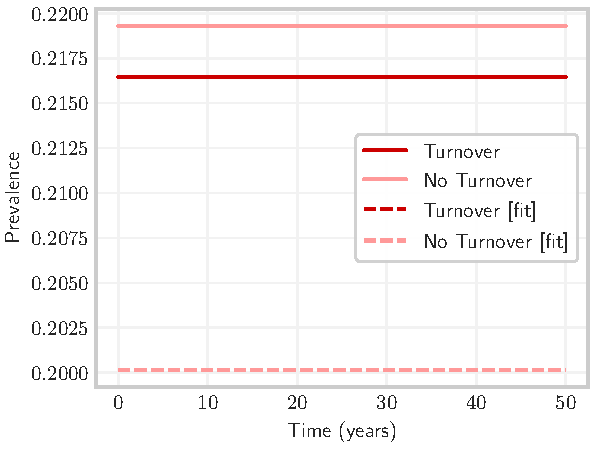
\includegraphics[width=\linewidth]{sit-tpaf-prevalence-high}
    \caption{High risk}
    \label{fig:tpaf-prevalence-high}
  \end{subfigure}
  \begin{subfigure}{0.45\linewidth}
    \centering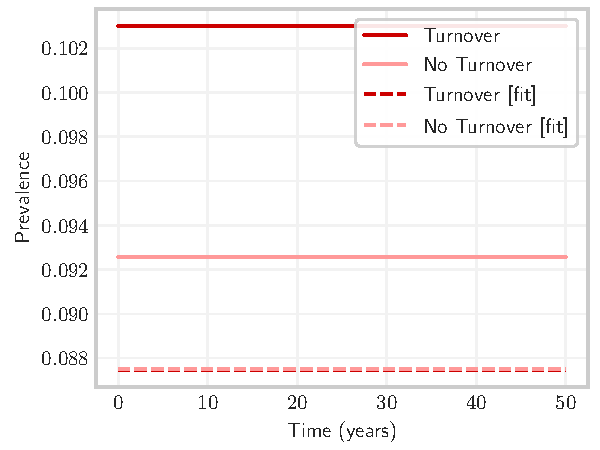
\includegraphics[width=\linewidth]{sit-tpaf-prevalence-med}
    \caption{Medium risk}
    \label{fig:tpaf-prevalence-med}
  \end{subfigure}
  \begin{subfigure}{0.45\linewidth}
    \centering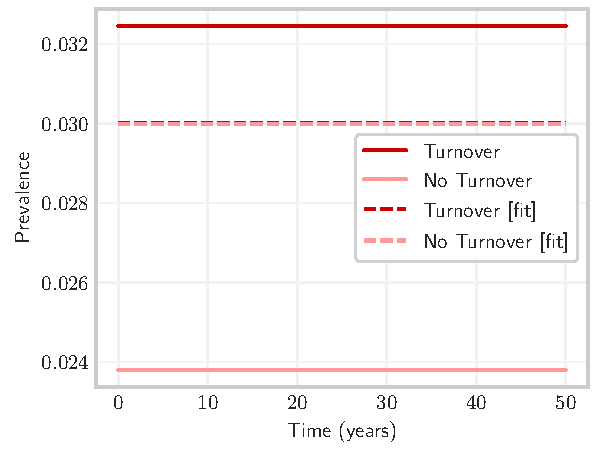
\includegraphics[width=\linewidth]{sit-tpaf-prevalence-low}
    \caption{Low risk}
    \label{fig:tpaf-prevalence-low}
  \end{subfigure}
  \begin{subfigure}{0.45\linewidth}
    \centering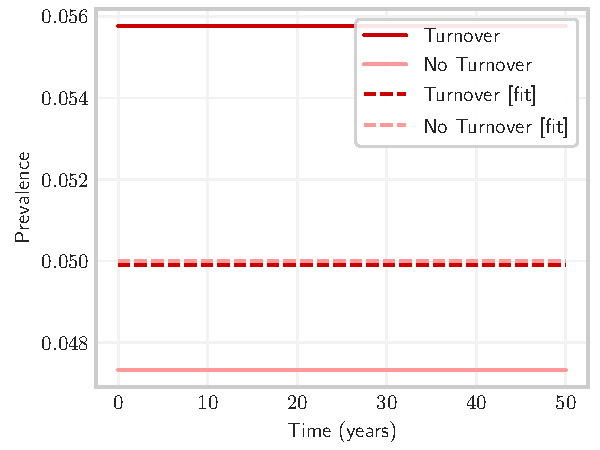
\includegraphics[width=\linewidth]{sit-tpaf-prevalence-all}
    \caption{Overall}
    \label{fig:tpaf-prevalence-all}
  \end{subfigure}
  \caption{Equilibrium STI prevalence among high, medium, and low risk groups as well as overall,
    with and without turnover,
    and with and without fitted $C_i$ to group-specific prevalence.}
  \label{fig:tpaf-prevalence}
\end{figure}
% ==================================================================================================
\subsection{Contact rate before and after model fitting}
\begin{figure}[H]
  \centering
  \begin{subfigure}{0.45\linewidth}
    \centering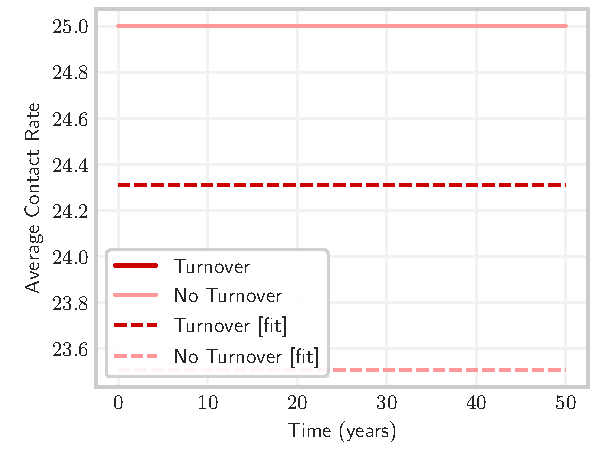
\includegraphics[width=\linewidth]{sit-tpaf-C-high}
    \caption{High risk}
    \label{fig:tpaf-C-high}
  \end{subfigure}
  \begin{subfigure}{0.45\linewidth}
    \centering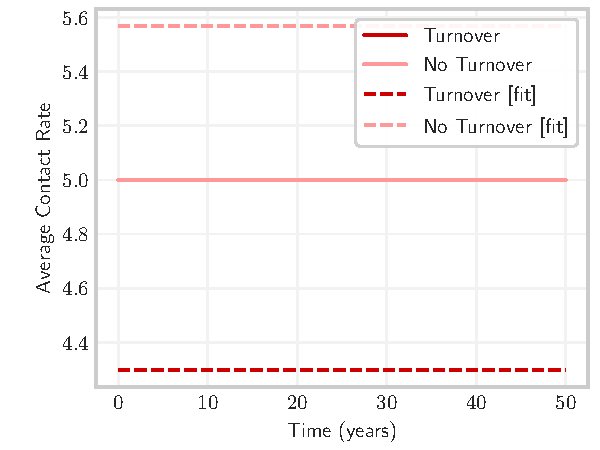
\includegraphics[width=\linewidth]{sit-tpaf-C-med}
    \caption{Medium risk}
    \label{fig:tpaf-C-med}
  \end{subfigure}
  \begin{subfigure}{0.45\linewidth}
    \centering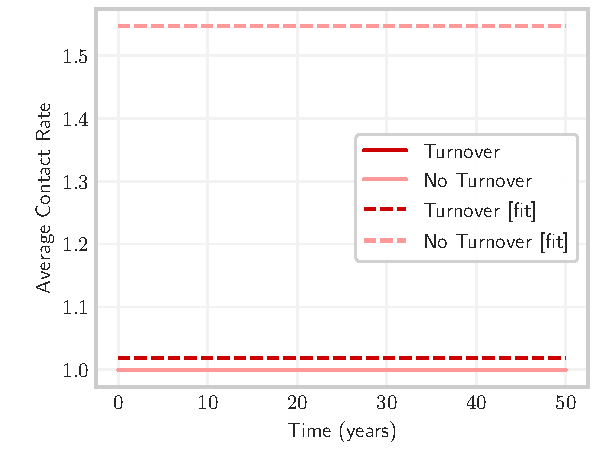
\includegraphics[width=\linewidth]{sit-tpaf-C-low}
    \caption{Low risk}
    \label{fig:tpaf-C-low}
  \end{subfigure}
  \begin{subfigure}{0.45\linewidth}
    \centering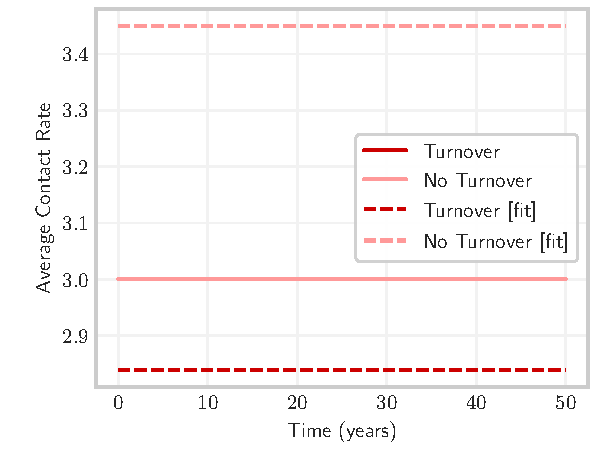
\includegraphics[width=\linewidth]{sit-tpaf-C-all}
    \caption{Overall}
    \label{fig:tpaf-C-all}
  \end{subfigure}
  \caption{Contact rates $C_i$ among high, medium, and low risk groups as well as overall,
    with and without turnover,
    and with and without model fitting to group-specific prevalence.}
  \label{fig:tpaf-C}
\end{figure}
% ==================================================================================================
\subsection{Influence of turnover on the TPAF of the highest risk group before model fitting}
\begin{figure}[H]
  \centering
  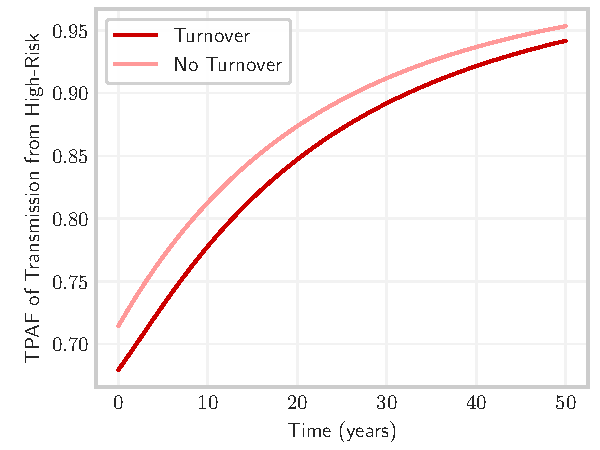
\includegraphics[width=0.45\linewidth]{sit-tpaf-tpaf-high-all-vs=raw}
  \caption{Transmission population attributable fraction (TPAF-from)
    of the high risk group in models with and without turnover,
    before model fitting.}
  \label{fig:tpaf-raw}
\end{figure}
% ==================================================================================================
\subsection{Distribution of health states at equilibrium}
\begin{figure}[H]
  \centering
  \begin{subfigure}{0.45\linewidth}
    \centering\includegraphics[width=\linewidth]{{1d-X-health-high-tau=0.1}.pdf}
    \caption{High Risk}
    \label{fig:1d-health-high}
  \end{subfigure}
  \begin{subfigure}{0.45\linewidth}
    \centering\includegraphics[width=\linewidth]{{1d-X-health-med-tau=0.1}.pdf}
    \caption{Medium risk}
    \label{fig:1d-health-med}
  \end{subfigure}
  \begin{subfigure}{0.45\linewidth}
    \centering\includegraphics[width=\linewidth]{{1d-X-health-low-tau=0.1}.pdf}
    \caption{Low Risk}
    \label{fig:1d-health-low}
  \end{subfigure}
  \begin{subfigure}{0.45\linewidth}
    \centering\includegraphics[width=\linewidth]{{1d-X-health-all-tau=0.1}.pdf}
    \caption{Overall}
    \label{fig:1d-health-all}
  \end{subfigure}
  \caption{Equilibrium health state proportions under different rates of turnover.}
  \label{fig:1d-health}
\end{figure}
% ==================================================================================================
\subsection{Rates of transition at equilibrium}
\label{aa:transitions}
\begin{figure}[H]
  \centering
  \begin{subfigure}{0.31\linewidth}
    \centering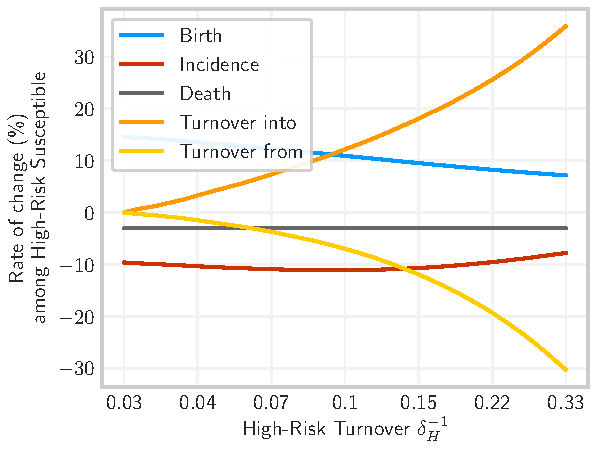
\includegraphics[width=\linewidth]{dX-high-S.pdf}
    \caption{High Risk Susceptible}\label{fig:dX-high-S}
  \end{subfigure}
  \begin{subfigure}{0.31\linewidth}
    \centering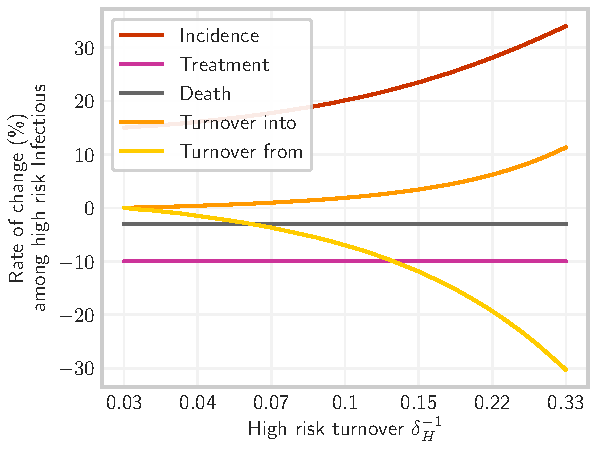
\includegraphics[width=\linewidth]{dX-high-I.pdf}
    \caption{High Risk Infectious}\label{fig:dX-high-I}
  \end{subfigure}
  \begin{subfigure}{0.31\linewidth}
    \centering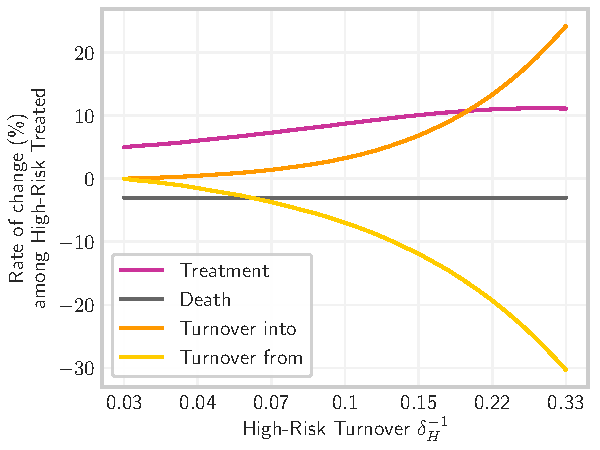
\includegraphics[width=\linewidth]{dX-high-T.pdf}
    \caption{High Risk Treated}\label{fig:dX-high-T}
  \end{subfigure}
  \begin{subfigure}{0.31\linewidth}
    \centering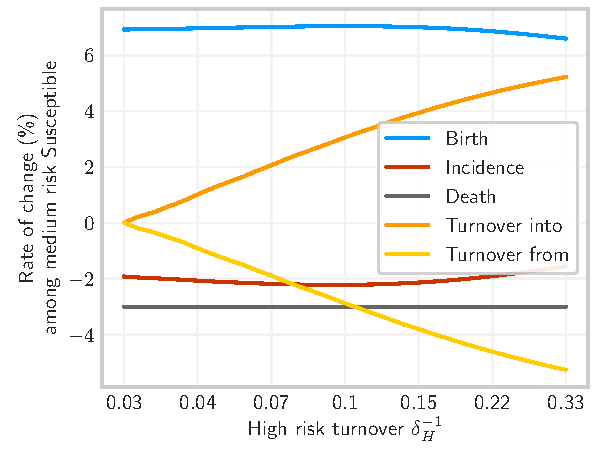
\includegraphics[width=\linewidth]{dX-med-S.pdf}
    \caption{Medium Risk Susceptible}\label{fig:dX-med-S}
  \end{subfigure}
  \begin{subfigure}{0.31\linewidth}
    \centering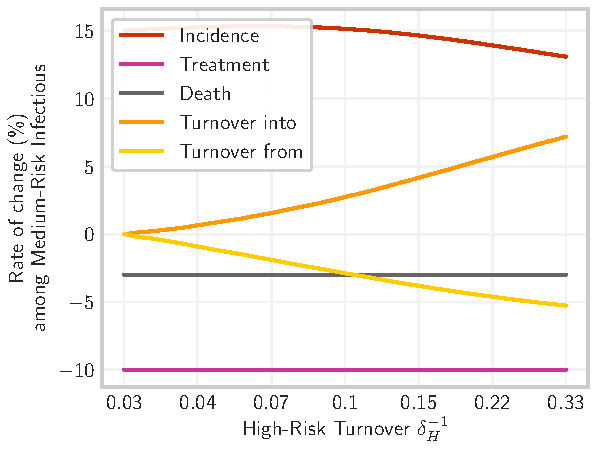
\includegraphics[width=\linewidth]{dX-med-I.pdf}
    \caption{Medium Risk Infectious}\label{fig:dX-med-I}
  \end{subfigure}
    \begin{subfigure}{0.31\linewidth}
    \centering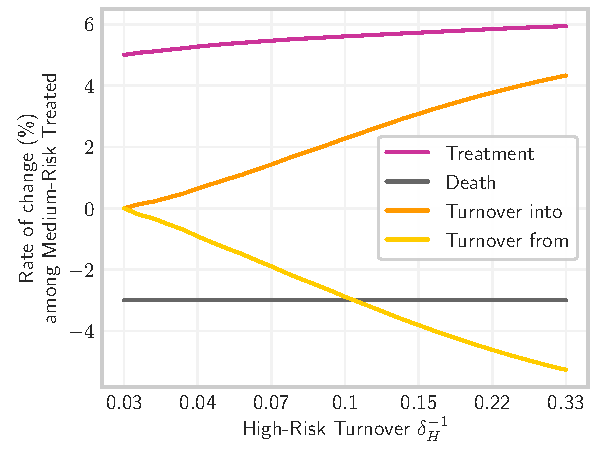
\includegraphics[width=\linewidth]{dX-med-T.pdf}
    \caption{Medium Risk Treated}\label{fig:dX-med-T}
  \end{subfigure}
  \begin{subfigure}{0.31\linewidth}
    \centering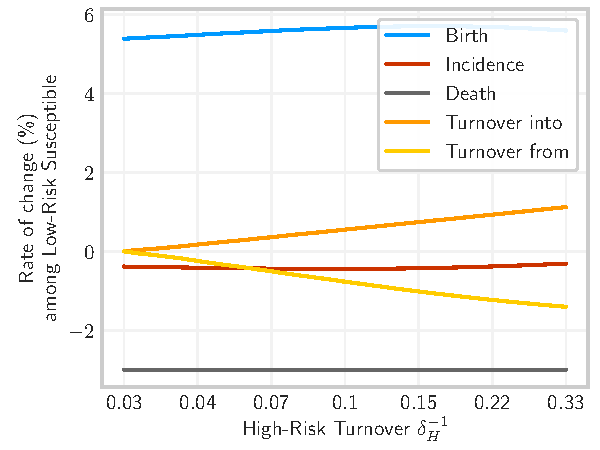
\includegraphics[width=\linewidth]{dX-low-S.pdf}
    \caption{Low Risk Susceptible}\label{fig:dX-low-S}
  \end{subfigure}
  \begin{subfigure}{0.31\linewidth}
    \centering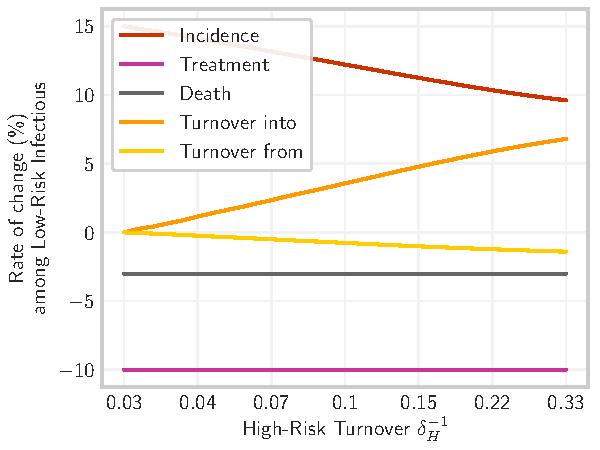
\includegraphics[width=\linewidth]{dX-low-I.pdf}
    \caption{Low Risk Infectious}\label{fig:dX-low-I}
  \end{subfigure}
  \begin{subfigure}{0.31\linewidth}
    \centering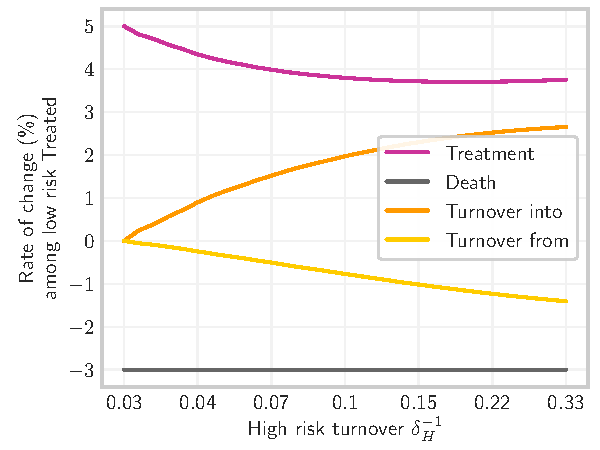
\includegraphics[width=\linewidth]{dX-low-T.pdf}
    \caption{Low Risk Treated}\label{fig:dX-low-T}
  \end{subfigure}
  \caption{Rates of transition among risk groups and health states at equilibrium.
    All transition rates are shown relative to the named group,
    for both afferent and efferent transitions.
    Although each system is at equilibrium,
    profiles should not sum to zero due population growth.}
\end{figure}
% ==================================================================================================
\subsection{New infections from turnover vs incidence}
\label{aa:inf-phi-vs-inc}
\begin{figure}[H]
  \centering\includegraphics[width=0.45\linewidth]{{2d-tip-all-tau=0.1}.pdf}
  \caption{Proportion of new infectious individuals in each risk group
    which are from turnover of infectious individuals,
    as opposed to infection of susceptible individuals in the risk group
    ($\tau = 0.1$).}
  \label{fig:new-inf-L}
\end{figure}